\documentclass[12pt,a5paper]{article}
\usepackage{xcolor}
\usepackage{pgfplots}
\usepackage{pgfplotstable}
\usepackage{tikz}

\pgfplotsset{compat=1.8}

\makeatletter
\pgfplotsset{
	/pgfplots/flexible xticklabels from table/.code n args={3}{%
		\pgfplotstableread[#3]{#1}\coordinate@table
		\pgfplotstablegetcolumn{#2}\of{\coordinate@table}\to\pgfplots@xticklabels
		\let\pgfplots@xticklabel=\pgfplots@user@ticklabel@list@x
	}
}
\makeatother

\definecolor{bblue}{HTML}{4F81BD}
\definecolor{rred}{HTML}{C0504D}
\definecolor{ggreen}{HTML}{9BBB59}
\definecolor{ppurple}{HTML}{9F4C7C}

\usepackage{graphicx}
\usetikzlibrary{positioning,arrows,shapes,fit,  shapes.geometric}



\pgfplotstableread[header=has colnames,
columns/TestSet/.style={string type},
]{%
TestSet	{Most Commonly Mentioned}	{ML Classical Feats.}	{ML Word Emb.}
ASOIAF	0.9140625	0.9765625	0.97265625
SOC	0.791208791	0.934065934	0.945054945
WOT	0.659722222	0.736111111	0.680555556
}{\res}

\renewcommand{\familydefault}{\sfdefault}


\begin{document}
\centering
\thispagestyle{empty}

{\Huge NovelPerpective\\}
{\Large Identifying Point of View Characters\\}
\vspace{0.3cm}
{\large Lyndon White, %
	Roberto Togneri, %
	Wei Liu, %
	Mohammed Bennamoun\\
}
\vspace{0.3cm}
\hspace{-1.5cm}
\begin{tikzpicture}
\begin{axis}[ybar,
	xticklabels from table={\res}{TestSet},
	legend style={at={(0.5,-0.3)}, anchor=north,legend columns=-1, draw=none},
%	enlargelimits=0.3,
	ymin = 0, ymax=1,
	enlarge x limits=0.3,
	xticklabel style={text width=8em, align=center},
	xtick = data,
	width=\textwidth, height= 4cm,
	bar width=0.6cm,
	yticklabel={\pgfmathparse{\tick*100}\pgfmathprintnumber{\pgfmathresult}\%},
	ytick = {0, 0.25, 0.50, 0.75, 1.00},
	ylabel = Accuracy,
	axis line style={draw=none},
	x tick style={draw=none},
	ytick pos=left,
]
\addplot[style={bblue,fill=bblue,mark=none}] table[x expr=\coordindex, y={ML Word Emb.}] {\res};
\addplot[style={rred,fill=rred,mark=none}] table[x expr=\coordindex, y={ML Classical Feats.}] {\res};
\addplot[style={ggreen,fill=ggreen,mark=none}] table[x expr=\coordindex, y={Most Commonly Mentioned}] {\res};
\legend{{Word Emb.},{Classical Feats.},{Baseline}}
\end{axis}
\end{tikzpicture}

\vspace{1cm}


\tikzset{
	every picture/.style={/utils/exec={\sffamily}},
	every matrix/.style={ampersand replacement=\&, rounded corners=10pt},
	every node/.style = {font=\small, inner sep = 3},
	>=latex,
	every text node part/.style={align=center}, auto,node distance=2.4, ->,
	every edge/.append style={every node/.style={font=\footnotesize}}
}


\resizebox{\textwidth}{!}{
	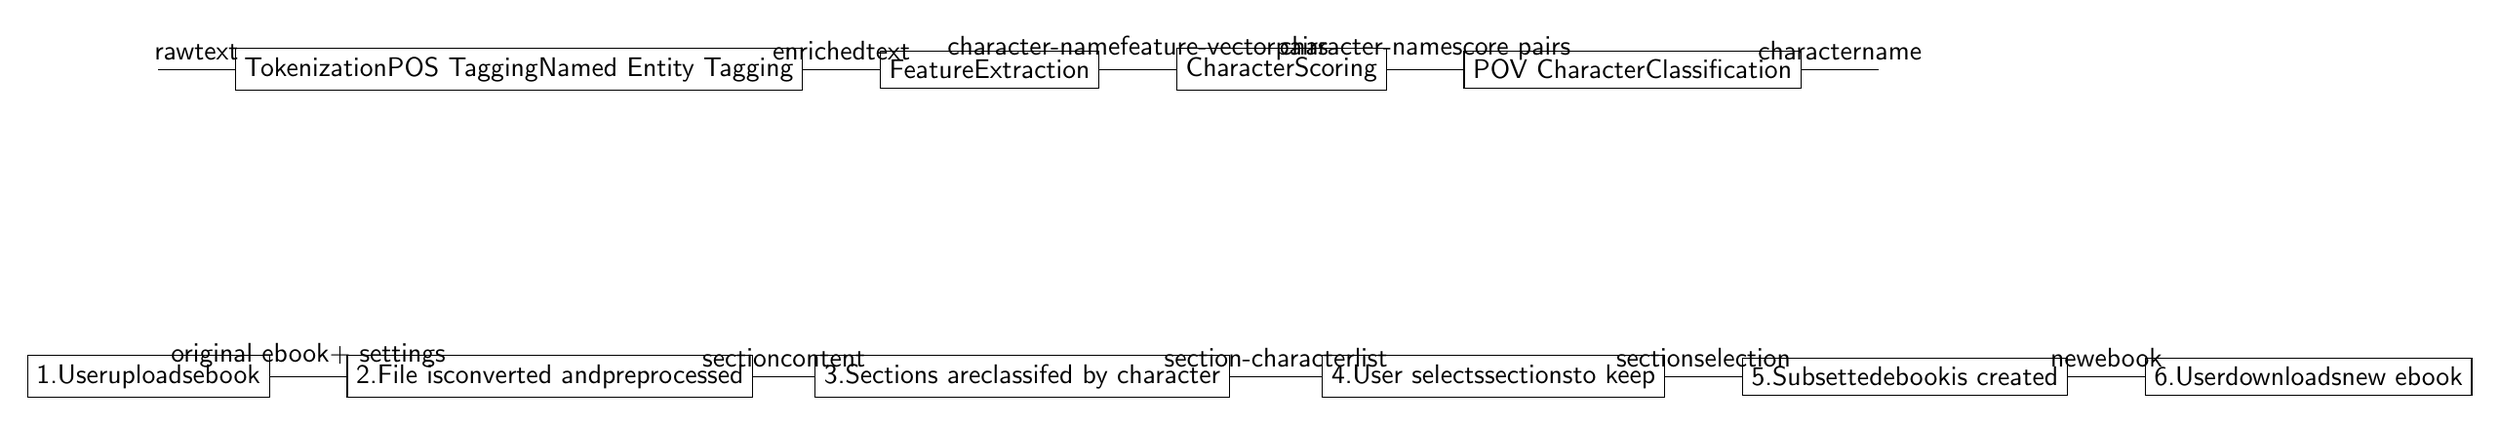
\begin{tikzpicture}	
	\begin{scope}[yshift=4cm]		
		\node(start1){};
		\node(enrich)[draw, right=of start1] {Tokenization\\POS Tagging\\Named Entity Tagging};
		\node(features)[draw, right=of enrich] {Feature\\ Extraction};
		\node(scoring)[draw, right=of features] {Character\\Scoring};				
		\node(classify)[draw, right=of scoring] {POV Character\\ Classification};
		\node(end)[right=of classify] {};
		
		\path (start1) edge node[above]{raw\\ text}  (enrich);
		\path (enrich) edge node[above]{enriched\\text} (features);
		\path (features) edge node[above]{character-name\\feature-vector\\pairs
		} (scoring);
		\path (scoring) edge node[above]{character-name\\score pairs
		} (classify);
		\path (classify) edge node[above]{character\\name}  (end);
	\end{scope}
		
	\node(start)[draw] {1.\\User\\ uploads\\ ebook};
	\node(convert)[draw, right=of start] {2.\\ File is\\ converted and \\preprocessed};
	\node(classify)[draw, right=of convert, xshift=-0.2cm] {3.\\Sections are \\ classifed by character};
	\node(select)[draw, right= of classify, xshift=0.2cm] {4.\\User selects\\ sections\\ to keep};
	\node(create)[draw, right=of select] {5.\\Subsetted\\ ebook\\ is created};
	\node(download)[draw, right=of create] {6.\\User \\downloads \\ new ebook};
	
	\path (start) edge[below] node[above]{original ebook \\ + settings}  (convert);
	\path (convert) edge[below] node[above]{section\\ content} (classify);
	\path (classify) edge[below] node[above]{section-character\\list} (select);
	\path (select) edge[below] node[above]{section\\selection}  (create);
	\path (create) edge[below] node[above]{new \\ ebook}  (download);	
	\end{tikzpicture}
}


\resizebox{\textwidth}{!}{

}



\end{document}